% Created 2021-10-06 mar 13:05
% Intended LaTeX compiler: pdflatex
%%% Local Variables:
%%% LaTeX-command: "pdflatex --shell-escape"
%%% End:
\documentclass[11pt]{article}
\usepackage[utf8]{inputenc}
\usepackage[T1]{fontenc}
\usepackage{graphicx}
\usepackage{grffile}
\usepackage{longtable}
\usepackage{wrapfig}
\usepackage{rotating}
\usepackage[normalem]{ulem}
\usepackage{amsmath}
\usepackage{textcomp}
\usepackage{amssymb}
\usepackage{listings}
\usepackage{capt-of}
\usepackage{hyperref}
\hypersetup{colorlinks=true, linkcolor=black}
\setlength{\parindent}{0in}
\usepackage[margin=1.1in]{geometry}
\usepackage[spanish]{babel}
\usepackage{mathtools}
\usepackage{palatino}
\usepackage{fancyhdr}
\usepackage{sectsty}
\usepackage{engord}
\usepackage{cite}
\usepackage{graphicx}
\usepackage{setspace}
\usepackage[compact]{titlesec}
\usepackage[center]{caption}
\usepackage{placeins}
\usepackage{tikz}
\usetikzlibrary{positioning}
\usetikzlibrary{bayesnet}
\usetikzlibrary{shapes.geometric}
\usetikzlibrary{decorations.text}
\usepackage{color}
\usepackage{amsmath}
\usepackage{minted}
\usepackage{pdfpages}
\usepackage[framemethod=TikZ]{mdframed} % Para entorno enunciado
\usepackage{amsthm}

\def\inline{\lstinline[basicstyle=\ttfamily,keywordstyle={}]}
\titlespacing*{\subsection}{0pt}{5.5ex}{3.3ex}
\titlespacing*{\section}{0pt}{5.5ex}{1ex}
\author{José Antonio Álvarez Ocete}
\date{\today}

% Comandos propios

\definecolor{myOrange}{rgb}{1, 0.733, 0.612}
\newcommand{\I}{\mathbb{I}}
\newcommand{\la}{\langle}
\newcommand{\ra}{\rangle}
\newcommand{\myparagraph}[1]{\paragraph*{ \\ #1}\mbox{}\\}
\newcommand{\R}{\mathbb{R}}
\newcommand{\E}{\mathbb{E}}
\newcommand{\Var}{\text{Var}}
%\newcommand{\log}{\text{log}}
% Para poner sonrisa sobre puntos suspensivos. Uso: \overplace{n}{\dotsc}
\newcommand{\overplace}[2]{%
	\overset{\substack{#1\\\smile}}{#2}%
}

\theoremstyle{plain}
\newtheorem*{theorem*}{Teorema}
\newtheorem{theorem}{Teorema}

\usepackage{mathtools}
\usepackage[shortlabels]{enumitem}
\DeclarePairedDelimiter\abs{\lvert}{\rvert}%
\usepackage{cancel}

%----------------------------------------------------------------------------------------
%	PACKAGES AND OTHER DOCUMENT CONFIGURATIONS
%----------------------------------------------------------------------------------------

\usepackage{blindtext} % Package to generate dummy text
\usepackage{charter} % Use the Charter font
\usepackage[utf8]{inputenc} % Use UTF-8 encoding
\usepackage{microtype} % Slightly tweak font spacing for aesthetics
\usepackage[english]{babel} % Language hyphenation and typographical rules
\usepackage{amsthm, amsmath, amssymb} % Mathematical typesetting
\usepackage{float} % Improved interface for floating objects
\usepackage[final, colorlinks = true, 
linkcolor = black, 
citecolor = black]{hyperref} % For hyperlinks in the PDF
\usepackage{graphicx, multicol} % Enhanced support for graphics
\usepackage{xcolor} % Driver-independent color extensions
\usepackage{marvosym, wasysym} % More symbols
\usepackage{rotating} % Rotation tools
\usepackage{censor} % Facilities for controlling restricted text
\usepackage{listings} % Environment for non-formatted code, !uses style file!
\usepackage{pseudocode} % Environment for specifying algorithms in a natural way
% Environment for f-structures, !uses style file!
\usepackage{booktabs} % Enhances quality of tables
\usepackage{tikz-qtree} % Easy tree drawing tool
% Configuration for b-trees and b+-trees, !uses style file!
%\usepackage[backend=biber,style=numeric,
%            sorting=nyt]{biblatex} % Complete reimplementation of bibliographic facilities
%\addbibresource{ecl.bib}
\usepackage{csquotes} % Context sensitive quotation facilities
\usepackage[yyyymmdd]{datetime} % Uses YEAR-MONTH-DAY format for dates
\renewcommand{\dateseparator}{-} % Sets dateseparator to '-'
\usepackage{fancyhdr} % Headers and footers
\pagestyle{fancy} % All pages have headers and footers
\fancyhead{}\renewcommand{\headrulewidth}{0pt} % Blank out the default header
\fancyfoot[L]{} % Custom footer text
\fancyfoot[C]{} % Custom footer text
\fancyfoot[R]{\thepage} % Custom footer text
\newcommand{\note}[1]{\marginpar{\scriptsize \textcolor{red}{#1}}} % Enables comments in red on margin

%-------------------------------
%	ENTORNO PARA ENUNCIADOS
%-------------------------------

%https://texblog.org/2015/09/30/fancy-boxes-for-theorem-lemma-and-proof-with-mdframed/
%\newcounter{enunciado}[section] - para resetear el counter por secciones
\newcounter{enunciado}
\setcounter{enunciado}{0}

% Esta línea pone la numeración de los ejercicios como {seccion}.{ejercicio}
%\renewcommand{\thetheo}{\arabic{section}.\arabic{enunciado}}
\newcommand{\thetheo}{\arabic{enunciado}}

\newenvironment{enunciado}[2][]{%
		\refstepcounter{enunciado}%
		\ifstrempty{#1}%
		{\mdfsetup{%
				frametitle={%
					\tikz[rounded corners, baseline=(current bounding box.east),outer sep=0pt]
					\node[anchor=east,rectangle,fill=myOrange]
					{\strut Ejercicio~\thetheo};}}
		}%
		{\mdfsetup{%
				frametitle={%
					\tikz[rounded corners, baseline=(current bounding box.east),outer sep=0pt]
					\node[anchor=east,rectangle,fill=myOrange]
					{\strut Ejercicio~\thetheo:~#1};}}%
		}%
		\mdfsetup{roundcorner=5pt, innertopmargin=10pt,linecolor=myOrange,%
			linewidth=2pt,topline=true,%
			frametitleaboveskip=\dimexpr-\ht\strutbox\relax
		}
		\begin{mdframed}[]\relax%
			%\label{#2}
	}
	{\end{mdframed}}

%-------------------------------
%	TITLE SECTION
%-------------------------------

\addtolength{\hoffset}{-2cm}
\addtolength{\textwidth}{4.1cm}
\addtolength{\voffset}{-2.25cm}
\addtolength{\textheight}{3cm}
\setlength{\parskip}{0pt}
\setlength{\parindent}{0in}

\begin{document}

\fancyhead[C]{}
\hrule \medskip % Upper rule
\begin{minipage}{0.295\textwidth} 
	\raggedright
	\footnotesize
	José Antonio Álvarez Ocete \hfill\\   
	77553417Q \hfill\\
	joseantonio.alvarezo@estudiante.uam.es
\end{minipage}
\begin{minipage}{0.4\textwidth} 
	\centering 
	\large 
	Entrega de problemas\\ 
	\normalsize 
	Teoría de la Información\\ 
\end{minipage}
\begin{minipage}{0.295\textwidth} 
	\raggedleft
	\today\hfill\\
\end{minipage}
\medskip\hrule 
\bigskip

%-------------------------------
%	CONTENTS
%-------------------------------

\begin{enunciado}
	
	Calcula la entropía de una variable $X \sim \text{N}(\mu, \sigma^2)$.
	
\end{enunciado}

Dada una variable aleatoria $X \sim \text{N}(\mu, \sigma^2)$, utilizamos la fórmula de la entropía para una variable contínua:

\[
	\begin{align*}
		H(X) & = - \E[log(X)] = - \int_\R f(x) \cdot \log_2 \bigg( \frac{1}{\sigma \sqrt{2\pi}} e^{\frac{-(x-\mu)^2}{2\sigma^ 2}} \bigg) dx \\
		& = - \int_\R f(x) \bigg( \log_2 \frac{1}{\sigma \sqrt{2\pi}} + \frac{-(x-\mu)^2}{2\sigma^ 2} \log_2 e \bigg) dx \\
		& = - \log_2 \frac{1}{\sigma \sqrt{2\pi}} \underbrace{\int_\R f(x) dx}_{= 1} + \frac{\log_2 e}{2\sigma^ 2} \underbrace{\int_\R f(x) (x-\mu)^2 dx}_{= \sigma^2} \\
		& = - \log_2 \frac{1}{\sigma \sqrt{2\pi}} + \frac{1}{2}\log_2 e \\
		& = \log_2 \sigma \sqrt{2\pi} + \frac{1}{2}\log_2 e \\
		& = \frac{1}{2} \log_2 2\pi\sigma^2  + \frac{1}{2}\log_2 e \\
		& = \frac{1}{2} \log_2 (2\pi\sigma^2 e) \\
	\end{align*}
\]
\qed

\begin{enunciado}
	
	Prueba que la información mútua entre dos variables aleatorias es simétrica. Esto es, $MI(X, Y) = MI(Y, X)$ para cualesquiera variables aleatorias $X,Y$.
	
\end{enunciado}

Lo probaremos para el caso discreto. Para el caso contínuo es equivalente utilizando la linealidad de la integral y los teoremas de Fubini y Tonelli. Utilizaremos el teorema de Bayes:

\begin{equation}
	\label{bayes}
	P(A|B) = \frac{P(A|B)}{P(B)}
\end{equation}

Partimos de la información mútua entre $X$ e $Y$, y llegaremos a la recíproca.

\[
	\begin{align*}
		MI(X, Y) & = -\sum_{x,y} P_{XY}(x,y) \log_2 \bigg( \frac{P_{X|Y}(x|y)}{P_X(x)} \bigg) \\
		& \stackrel{(\ref{bayes})}{=} -\sum_{x,y} P_{XY}(x,y) \log_2 \bigg( \frac{P_{XY}(x,y)}{P_X(x) P_Y(y)} \bigg) \\
		& \stackrel{(\ref{bayes})}{=} -\sum_{x,y} P_{XY}(x,y) \log_2 \bigg( \frac{P_{Y|X}(y|x)}{P_Y(y)} \bigg) = MI(Y, X)\\
	\end{align*}
\]
\qed

\begin{enunciado}
	
	Prueba la siguiente identidad entre información mútua y entropías: $MI(X, Y) = H(X) + H(Y) - H(X, Y)$.
	
\end{enunciado}

Lo probaremos para el caso discreto. Para el caso contínuo es equivalente utilizando la linealidad de la integral y los teoremas de Fubini y Tonelli. Para este y otros ejercicios utilizaremos una igualdad que conviene probar por separado. Es la siguiente, fijado un $x \in X$:

\begin{equation}
	\label{truco}
	\sum_y P_{XY}(x,y) = P_X(x)
\end{equation}

Probar esta igualdad es sencillo:

\[
	\sum_y P_{XY}(x,y) \stackrel{(\ref{bayes})}{=} \sum_y P_{Y|X}(y|x) P_X(x) = P_X(x) \underbrace{\sum_y P_{Y|X}(y|x)}_{= 1} = P_X(x)
\]

Para demostrar la igualdad pedida, partimos de la información mútua y operamos de la siguiente forma:

\[
	\begin{align*}
	MI(X, Y) & = - \sum_{x,y} P_{XY}(x,y) \log_2 \bigg( \frac{P_{XY}(x,y)}{P_X(x) P_Y(y)} \bigg) \\
	& = - \sum_{x,y} P_{XY}(x,y)  \bigg( \log_2 P_{XY}(x,y) - \log_2 P_X(x) - \log_2 P_Y(y) \bigg) \\
	& = - \sum_{x,y} P_{XY}(x,y) \log_2 P_{XY}(x,y) + \sum_{x,y} P_{XY}(x,y) \log_2 P_X(x) +\sum_{x,y} P_{XY}(x,y) \log_2 P_Y(y) \\
	& \stackrel{(\ref{truco})}{=} - \sum_{x,y} P_{XY}(x,y) \log_2 P_{XY}(x,y) + \sum_{x} P_X(x) \log_2 P_X(x) +\sum_{y} P_Y(y) \log_2 P_Y(y) \\
	& = - H(X, Y) + H(X) + H(Y)
	\end{align*}
\]
\qed


\begin{enunciado}
	
	Prueba las siguientes identidades.
	
	\begin{itemize}
		\item $H(X, Y) = H(X) + H(Y|X) = H(Y) + H(X|Y)$
		\item $MI(X, Y) = H(X) - H(X|Y) = H(Y) - H(Y|X)$
		\item $MI(X, X) = H(X)$
	\end{itemize}
	
\end{enunciado}

Probaremos estas igualdades para el caso discreto. Para el caso contínuo son equivalentes utilizando la linealidad de la integral y los teoremas de Fubini y Tonelli. Partimos de la entropía condicionada: 

\[
	\begin{align*}
		H(Y|X) & = - \sum_x P_X(x) \sum_y P_{Y|X}(y|x) \log_2 P_{Y|X}(y|x) \\
		& \stackrel{(\ref{bayes})}{=} - \sum_x P_X(x) \sum_y \frac{P_{X,Y}(x,y)}{P_X(x)} \log_2 \frac{P_{X,Y}(x,y)}{P_X(x)} \\
		& = - \sum_x \frac{P_X(x)}{P_X(x)} \sum_y P_{X,Y}(x,y) \bigg( \log_2 P_{X,Y}(x,y) - \log_2 P_X(x) \bigg) \\
		& = - \sum_{x,y} P_{X,Y}(x,y) \bigg( \log_2 P_{X,Y}(x,y) - \log_2 P_X(x) \bigg) \\
		& = - \sum_{x,y} P_{X,Y}(x,y) \log_2 P_{X,Y}(x,y) + \sum_{x,y} P_{X,Y}(x,y)\log_2 P_X(x) \\
		& \stackrel{(\ref{truco})}{=} - \sum_{x,y} P_{X,Y}(x,y) \log_2 P_{X,Y}(x,y) + \sum_x P_X(x)\log_2 P_X(x) \\
		& = H(X,Y) - H(X) 
	\end{align*}
\]

Pasamos $H(X)$ al otro miembro sumando y obtenemos la primera igualdad buscada:

\begin{equation}
	\label{entropies}
	H(X,Y) = H(X) + H(Y|X)
\end{equation}
\qed

Para probar la segunda igualdad haremos uso de la primera:

\[
	\begin{align*}
		MI(X,Y) & = H(X) + H(Y) - H(X,Y) \\
		 & \stackrel{(\ref{entropies})}{=} H(X) + H(Y) - (H(Y) + H(X|Y)) \\
		 & = H(X) - H(X|Y)
	\end{align*}
\]
\qed

Para probar la tercera igualdad necesitaremos un hacer uso de un resultado intermedio: La entropía de una variable aleatoria condicionada a sí misma es nula. Esto encaja con nuestra intuición, pues al fijar una variable aleatoria, la sorpresa asociada a la medición de la misma es trivial. Probemos este resultado intermedio:

\[
	\begin{align*}
		H(X|X) & = - \sum_{x_1} P_X(x_1) \sum_{x_2} P_{X|X}(x_2|x_1) \log_2 P_{X|X}(x_2|x_1) \\
		&  = - \sum_{x_1} P_X(x_1) P_{X|X}(x_1|x_1) \underbrace{\log_2 P_{X|X}(x_1|x_1)}_{= 0} = 0
	\end{align*}
\]

Donde hemos usado que:

\[
	P_{X|X}(x_2|x_1) =
	\begin{cases*}
		0 \quad \text{si } x_1 \neq x_2 \\
		1 \quad \text{si } x_1 = x_2
	\end{cases*}
\]

Conociendo este resultado, probar la igualdad pedida es sencillo:

\[
	\begin{align*}
		MI(X,X) & = H(X) + H(X) - H(X,X) \\
		& \stackrel{(\ref{entropies})}{=} 2 H(X) - (H(X) - \underbrace{H(X|X)}_{= 0}) = H(X)
	\end{align*}
\]
\qed

\begin{enunciado}
	
	Probar que en el ámbito del \emph{temporal encoding} y suponiendo $\triangle t \ll 1/r$, entonces la entropía es:
	
	\[
		H \approx Tr \log_2(\frac{e}{r \triangle t})
	\]
\end{enunciado}

Antes de probar la igualdad requerida especificaremos una serie de definiciones naturales en el contexto del \emph{temporal encoding}:

Dado un tren de \emph{spikes} y un tamaño de ventana $\triangle t$, asignaremos un $1$ a la ventana si hay un spike en ella y un $0$ si no:

\begin{figure}[H]
	\centering
	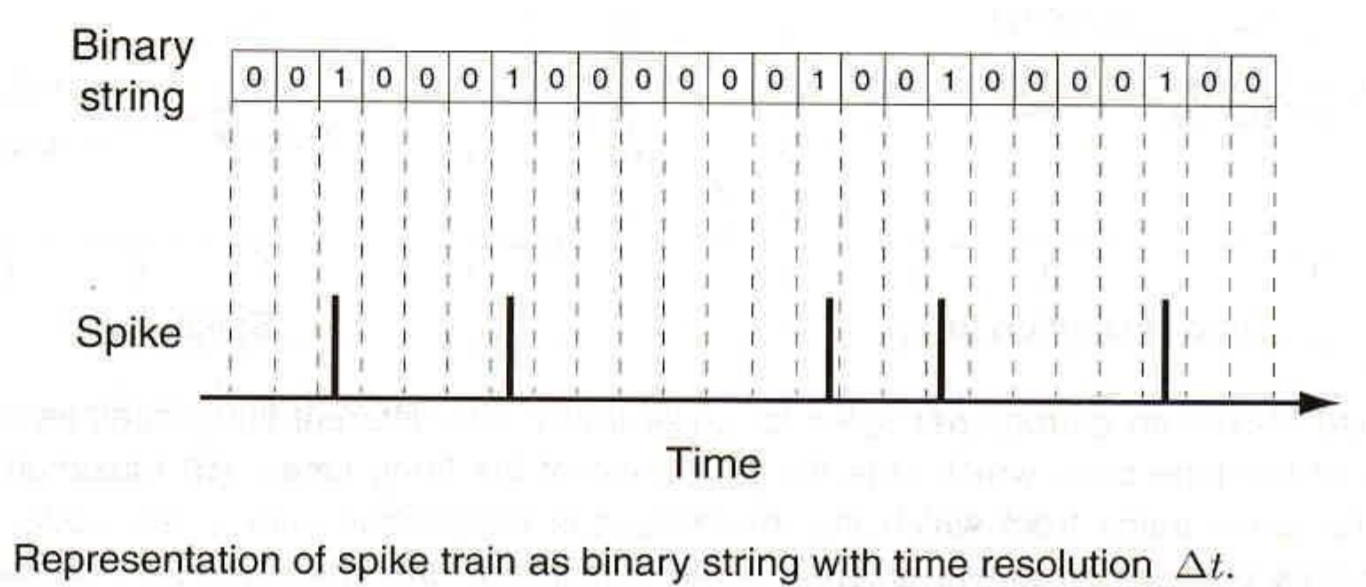
\includegraphics[scale=0.5]{figures/temporal_encoding.PNG}
	\caption{Ejemplo de temporal encoding}
\end{figure}

Denominaremos \emph{tren de spikes} a un conjunto de $T$ valores $0/1$ de nuestra serie temporal, donde $T$ es un número natural fijo. De esta forma, el número total de ventanas será $N = T/\triangle t$. \\

Adicionalmente, definimos el \emph{firing rate} $r$ como el número medio de spikes por tren de spikes:

\[
	r = \frac{\#spikes}{T}
\]

Estudiémos a continuación nuestra hipótesis $\triangle t \ll 1/r$. Podemos reescribirla de la siguiente forma:

\[
	\triangle t \ll \frac{1}{r} \iff r \triangle t \ll 1
\]

Por otro lado, podemos estudiar la probabilidad de obtener un spike en una ventana aleatoria. Esto es:

\[
	P[\text{spike en ventana}] \equiv P = \frac{\#spikes}{M} = \frac{\#spikes}{T / \\
		 t} = \triangle t \cdot \frac{\#spikes}{T} = r \triangle t
\]

Es decir, nuestra hipótesis se traduce en que la probabilidad de encontrar un spike en una ventana sea mínima. Siempre podemos asegurar que este valor sea arbitrariamente pequeño mediante el valor del parámetro $\triangle t$, por lo que siempre podemos asegurar esta hipótesis. \\

Para estimar la entropía hemos de conocer la probabilidad de ocurrencia de cada evento. Para ello supondremos que extraemos un tren de spikes aleatoria y uniformemente entre todas las cadenas posibles. Consecuentemente, cada posible evento $x_i$ tendrá probabilidad de ocurrencia el inverso del número de cadenas posibles con ese número de $0$s y $1$s:

\[
	P(x_i) = \frac{1}{\binom{N}{Tr}} \quad i \in \{1, \ldots, \binom{N}{Tr}\}
\]

Denominamos al número de spikes $N_1 \equiv \#spikes = Tr$ al número de spikes o número de $1$, y $N_0 = N - N_1$ al número de $0$s. Dado que los sucesos son equiprobables, la entropía de un suceso viene dada por el logaritmo del número total de eventos denominado $E$:

\[
	\begin{align*}
		H & = \sum_x \underbrace{P(x)}_{= 1/E} * \log_2 \frac{1}{P(x)} \\
		& = E \sum_x * \log_2 \frac{1}{1 / E} \\
		& = \frac{1}{E} \sum_x * \log_2 \frac{1}{1 / E} \\
		& = \frac{1}{E} E \log_2 E \\
		& = \log_2 E \\
		& = \log_2 \binom{N}{N_1} \\
		& = \frac{1}{\log 2} \bigg( \log N! - \log N_0! - log N_1! \bigg)
	\end{align*}	
\]

donde hemos hecho uso del logaritmo natural. A continuación hemos de hacer uso de la \href{https://en.wikipedia.org/wiki/Stirling\%27s_approximation}{aproximación de Stirling} para obtener una expresión del logaritmo de un número factorial:

\[
	\log n! = n \log n - n + O(\log n)
\]

Donde el término logaritmo $O(\log n)$ es despreciable frente a los polinómicos cuando $n \rightarrow \infty$. En particular, aproximaremos el susodicho valor por:

\[
	\log n! \approx n \log n - n = n (\log n - 1)
\]

Utilizando esta aproximación y sabiendo que $N = N_0 + N_1$ obtenemos:

\[
	\begin{align*}
		H & = \frac{1}{\log 2} \bigg( \log N! - \log N_0! - log N_1! \bigg) \\
		& \approx \frac{1}{\log 2} \bigg( N (\log N - 1) - N_0 (\log N_0 - 1) - N_1 (log N_1 - 1) \bigg) \\
		& = \frac{1}{\log 2} \bigg( N \log N + N_0 \log N_0  + N_1 log N_1 + (N_0 + N_1 - N) \bigg) \\
		& = \frac{1}{\log 2} \bigg( N_0 (\log N - \log N_0) + N_1 (\log N - \log N_1) \bigg) \\
		& = - \frac{N}{\log 2} \bigg( \frac{N_0}{N} \log \frac{N_0}{N} + \frac{N_1}{N} \log \frac{N_1}{N} \bigg) \\
		& = - \frac{N}{\log 2} \bigg( \frac{N_0}{N} \log \frac{N_0}{N} + \frac{N_1}{N} \log \frac{N_1}{N} \bigg) \\
		& = - \frac{N}{\log 2} \bigg( (1-P) \log (1-P) + P \log P \bigg) \\
	\end{align*}	
\]

Pues $P = N_1/N$ y $1 - P = N_0/N$. Finalmente, volvemos a los parámetros originales recordando que $r \triangle t = P$ y $M = T / \triangle t$:

\[
	\begin{align*}
		H & \approx - \frac{T}{\triangle t \log 2} \bigg( (1 - r\triangle t) \log (1 - r\triangle t) + r\triangle t \log (r\triangle t) \bigg) \\
	\end{align*}	
\]

Finalmente utilizamos el desarrollo en serie de Taylos de la función $log(1 + x)$, donde $x = -r\triangle t$. Utilizando nuestra hipótesis $\triangle t \ll 1/r$ podemos despreciar los términos de orden superior. Sustituyendo en la expresión anterior obtenemos:

\[
	\begin{align*}
		H & \approx - \frac{T}{\triangle t \log 2} \bigg( r\triangle t \log (r\triangle t) + (1 - r\triangle t) (- r\triangle t) \bigg) \\
		& \approx - \frac{T}{\triangle t \log 2} \bigg( r\triangle t \log (r\triangle t) - r\triangle t \bigg) \\
		& = - \frac{T \cdot r\triangle t}{\triangle t \log 2} (\log (r\triangle t) - 1) \\
		& = - \frac{Tr}{\log 2} (\log (r\triangle t) - \log e) \\
		& = \frac{Tr}{\log 2} \log \frac{e}{r\triangle t} \\
		& = Tr \log_2 \frac{e}{r\triangle t}
	\end{align*}
\]
\qed

\begin{enunciado}
	
	Prueba la siguiente identidad: $H(X, Y|Z) = H(X|Z) + H(Y|X, Z)$.
	
\end{enunciado}

Lo probaremos para el caso discreto. Para el caso contínuo es equivalente utilizando la linealidad de la integral y 	los teoremas de Fubini y Tonelli. Haremos uso del teorema de Bayes para varias variables:

\begin{equation}
	\label{bayes2}
	P(A, B | C) = P(A|C) \cdot P(B|A, C)
\end{equation}

Recordemos las definiciones de entropías para varias variables que aparecen en el enunciado:

\[
	\begin{align*}
		H(X, Y | Z) & = - \sum_{x,y,z} P_{XYZ}(x,y,z) \log_2 P_{XY|Z}(x, y|z) \\
		H(X|Z) & = - \sum_z P_Z(z) \sum_x P_{X|Z}(x|z) \log_2 P_{X|Z}(x|z) \\
		H(Y |X, Z) & = - \sum_{x,z} P_{XZ}(x,z) \sum_y P_{Y|XZ}(y|x,z) \log_2 P_{Y|XZ}(y|x,z)
	\end{align*}
\]

Obtenemos la siguiente cadena de igualdades:

\[
	\begin{align*}
		H(X, Y | Z) & = - \sum_{x,y,z} P_{XYZ}(x,y,z) \log_2 P_{XY|Z}(x, y|z) \\
		& \stackrel{(\ref{bayes2})}{=} - \sum_{x,y,z} P_{XYZ}(x,y,z) \log_2 \bigg( P_{X|Z}(x|z) \cdot P_{Y|XZ}(y|x,z) \bigg) \\
		& = - \sum_{x,y,z} P_{XYZ}(x,y,z) \bigg( \log_2 P_{X|Z}(x|z) + \log_2 P_{Y|XZ}(y|x,z) \bigg) \\
		& = \underbrace{- \sum_{x,y,z} P_{XYZ}(x,y,z) \log_2 P_{X|Z}(x|z)}_{(A)} \underbrace{- \sum_{x,y,z} P_{XYZ}(x,y,z) \log_2 P_{Y|XZ}(y|x,z)}_{(B)} 
	\end{align*}
\]

Resta probar que los términos $(A)$ y $(B)$ son $H(X|Z)$ y $H(Y|X, Z)$ respectivamente:

\[
	\begin{align*}
		(A) & = - \sum_{x,y,z} P_{XYZ}(x,y,z) \log_2 P_{X|Z}(x|z) \\
		& = - \sum_{x,z} \log_2 P_{X|Z}(x|z) \sum_y P_{XYZ}(x,y,z)  \\
		& \stackrel{(\ref{truco})}{=} - \sum_{x,z} P_{XZ}(x,z) \log_2 P_{X|Z}(x|z) \\
		& \stackrel{(\ref{bayes})}{=} - \sum_{x,z} P_{X|Z}(x|z) P_Z(z) \log_2 P_{X|Z}(x|z) \\
		& = - \sum_z P_Z(z) \sum_x P_{X|Z}(x|z) \log_2 P_{X|Z}(x|z) = H(X|Z)
	\end{align*}
\]

\[
	\begin{align*}
		(B) & = - \sum_{x,y,z} P_{XYZ}(x,y,z) \log_2 P_{Y|XZ}(y|x,z) \\
		& \stackrel{(\ref{bayes})}{=} - \sum_{x,y,z} P_{Y|XZ}(y|x,z) P_{XZ}(x,z) \log_2 P_{Y|XZ}(y|x,z) \\
		& = - \sum_{x,z} P_{XZ}(x,z) \sum_y P_{Y|XZ}(y|x,z) \log_2 P_{Y|XZ}(y|x,z) = H(Y|X, Z)
	\end{align*}
\]
\qed

\end{document}

